\subsection{UC-15 Algoritmo per selezionare i partecipanti}
Selezione degli utenti iscritti ad un evento con strategia Greedy.
\\
\\
\textit{Breve Descrizione: Se il numero di iscritti ad un evento eccede il numero massimo di partecipanti, vengono selezionati in base alla loro esperienza.} 
\\
\\
\textit{Attori Coinvolti:Sistema, Organizzatore}
\\
\\
\textit{Precondizione: L'utente organizzatore avvia la funzione di selezione degli utenti iscritti ad un proprio evento.}
\\
\\
\textit{Postcondizione: Gli utenti non selezionati vengono eliminati dai partecipanti dell'evento e viene restituita una lista degli utenti confermati.}
\\
\\
\textit{Procedimento:}
\begin{enumerate}
	\item L'utente organizzatore accede all'app e seleziona un evento che ha creato;
 	\item L'opzione 'Seleziona partecipanti' viene selezionata.
	\item L'algoritmo viene applicato sulla lista degli iscritti all'evento.
\end{enumerate}



\textit{FlowChart (\ref*{fig:FlowChart}) e pseudocodice: L'approccio si basa sull'idea di selezionare in modo iterativo gli utenti con il livello più
adatto, iniziando dal livello dell'evento e ampliando la ricerca ai livelli adiacenti solo se
necessario.}

% Impostazioni per lo pseudocodice
\lstset{
    language=Java, % Imposta il linguaggio del codice
    basicstyle=\ttfamily\small, % Stile di base del testo
    keywordstyle=\color{blue}, % Stile delle parole chiave
    commentstyle=\color{gray}, % Stile dei commenti
    stringstyle=\color{red}, % Stile delle stringhe
    numbers=left, % Posizione dei numeri di riga
    numberstyle=\tiny, % Stile dei numeri di riga
    stepnumber=1, % Passo tra i numeri di riga
    tabsize=2, % Dimensione del tab
    showspaces=false,
    showstringspaces=false,
    breaklines=true, % Permette di spezzare le righe troppo lunghe
    breakatwhitespace=true,
}
\begin{lstlisting}
algoritmo selezionaIscritti(Lista listaIscritti) 
    S <- {}
    limiteMax = Event.maxPeople
    
    if (listaIscritti.dim <= limiteMax) then S <- all(listaIscritti)
    else 
        livello = Event.level
        int i = 0  //posti occupati
        int j = 0  //distanza dal livello evento
        
        while((i != limiteMax) and (listaIscritti != {})) do
            utenteConfermato = seleziona(listaIscritti, livello, j)
            
	    if(utenteConfermato != null) {
            	listaIscritti <- listaIscritti / {utenteConfermato}
            	S <- S U {utenteConfermato}
            	i + 1
	    }

            if(not listaIscritti.contains(anotherUser con userLevel = livello +- j)) then j+1
        
    return S

//prima vengono considerati gli utenti con lo stesso livello dell'evento
//poi quelli ai livelli +-1, +-2 fino a esaurimento posti
funzione seleziona(listaIscritti, livello, distanza)
    return (User con userLevel = livello + distanza) or (User con userLevel - distanza)
\end{lstlisting}

\begin{figure}[ht!]
    \centering
    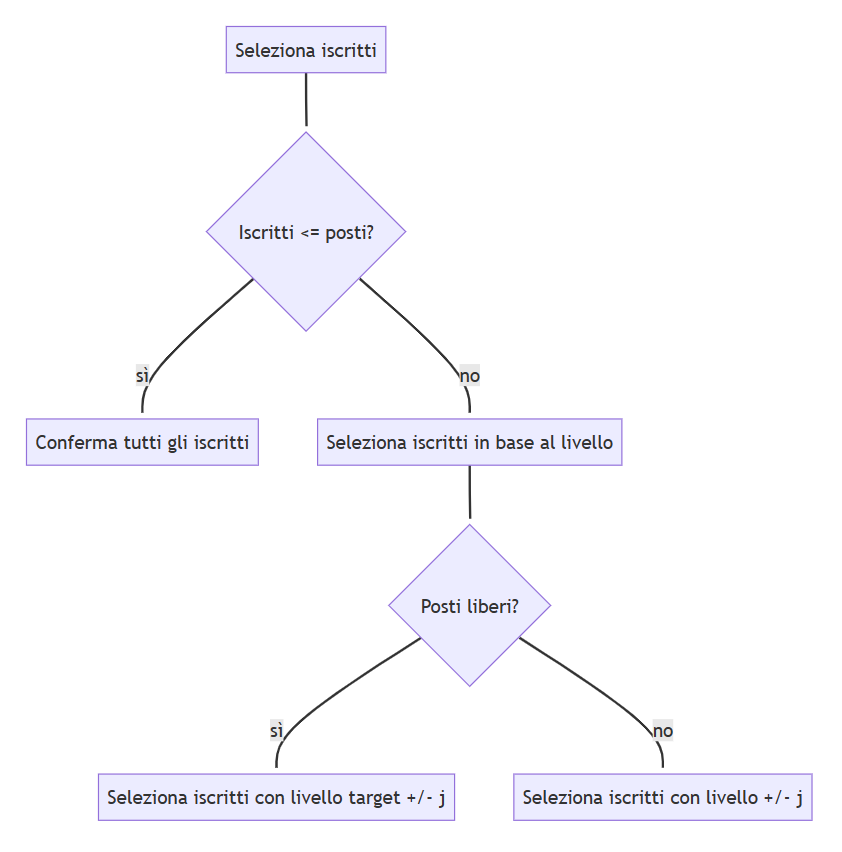
\includegraphics[width = 0.5\textwidth]{Iterazione 2/images/flowchart.png}
    \caption{FlowChart}
	\label{fig:FlowChart}
\end{figure}

\textit{Analisi di Complessità: l'algoritmo ha una complessità temporale più significativa rispetto a quella spaziale, la sua efficienza dipende dal rapporto tra il numero massimo di posti disponibili e la dimensione totale della lista degli iscritti.}
\begin{enumerate}
	\item Complessità temporale: 
        \begin{itemize}
            \item Caso Migliore (Numero di iscritti <= Numero massimo di posti):
                Nel caso in cui il numero di iscritti sia inferiore o uguale al numero massimo di posti disponibili, l'algoritmo esegue una copia di tutti gli iscritti nella lista `S`.
                Complessità Temporale: O(n), dove n è la dimensione della lista degli iscritti.
            \item Caso Peggiore (Numero di iscritti > Numero massimo di posti):
                Nel caso in cui il numero di iscritti superi il numero massimo di posti, l'algoritmo utilizza due cicli while annidati. Il ciclo esterno viene eseguito fino a quando non vengono occupati tutti i posti desiderati o la lista degli iscritti è vuota, mentre il ciclo interno verifica la presenza di utenti con il livello desiderato nella lista degli iscritti.
                Nel peggiore dei casi, il numero di iterazioni del ciclo esterno è limitato dal numero massimo di posti e dalla dimensione della lista degli iscritti.
                Complessità Temporale: O(limiteMax * n), dove n è la dimensione della lista degli
                iscritti.
        \end{itemize}
	\item Complessità spaziale: 
        \begin{itemize}
            \item Spazio Ausiliario (Variabili e Strutture Dati): La lista `S` contiene gli             iscritti selezionati. Nel caso peggiore, sarà di dimensione`limiteMax`.
            \item Altre variabili ausiliarie occupano uno spazio costante.
        \end{itemize}    
            Complessità Spaziale: O(limiteMax).
\end{enumerate}


